\section{Video}
Un video viene percepito dal nostro sistema visivo con la \textbf{persistenza della visione}, e per ottenere il movimento apparente (serie di immagini statiche) è necessario individuare la frequenza minima per avere una visione continua. 

La persistenza della visione è un fenomeno per il quale un'immagine rimane per qualche frazione di secondo in memoria, attribuito a livello cerebrale. Ciò permette di ottenere un movimento continuo. 

Esistono frequenze di campionamento prestabilite per percepire una serie di immagini come un video continuo:
\begin{itemize}
	\item Una teleconferenza è a 10 fps;
	\item Un film muto è a 16 fps (\textit{limite del movimento a scatti});
	\item Un film sonoro è a 24 fps;
	\item Le televisioni sono a 25-60 fps, a seconda della tipologia.
\end{itemize}

Dalla conoscenza della risposta si determina la progettazione di un dispositivo di riproduzione video. La risposta dell'HVS dipende dal contenuto frequenziale, rispetto al tempo e allo spazio.

Per definire il numero di immagini al secondo (\textit{frame rate} e \textit{refresh rate}) bisogna definire una \textbf{soglia critica} legata alla frequenza di Flicker, ottenuta in base a una serie di parametri, quindi variabile nel tempo e nello spazio.

Se la frequenza è troppo alta, l'immagine non è più nitida: il range ha anche un limite superiore, con estremi tra i 20 e gli 80 Hz, definendo una \textit{Critical Flicker Frequency} alla quale lo stimolo passa da intermittente a continuo. Essa varia in funzione di:
\begin{itemize}
	\item Luminosità media del display;
	\item Luminosità dell'ambiente;
	\item Distanza dallo schermo.
\end{itemize}

Un \textbf{video field} è un insieme di campioni in un'immagine, composto da linee alternate. I vari field sono campionati a istanti diversi. L'aumento delle frequenza di refresh per la televisione è ottenuto dividendo l'immagine in due campi, le cui righe non vengono scansionate sequenzialmente ma sono \textbf{alternate tra pari e dispari}. Il refresh include anche la ripetizione della stessa immagine, riducendo il flicker.

La \textbf{scansione progressiva} consiste nella trasmissione in sequenza e in modo continuo di tutte le linee. Al contrario, la \textbf{scansione interlacciata} divide il frame in field trasmessi in metà del tempo totale.

I 24 fps del cinema non sono sempre sufficienti, quindi i proiettori possono arrivare a 48 o addirittura 72. Nella trasmissione analogica, invece, la frequenza viene virtualmente raddoppiata con l'interfacciamento: le risposte in frequenza vengono combinate. Nei display dei computer si utilizza un rate di 72 fps.

Il sottocampionamento introduce aliasing quando il movimento è molto veloce, causando differenze di percezione ovviate da opportuni filtri passa-basso (\textit{smoothing}). 

\subsection{Riproduzione}
Un segnale \textit{analogico} ha risoluzione definita dal \textbf{numero di linee di scansione}. \\
Un segnale \textit{digitale} ha risoluzione definita dal \textbf{numero di pixel}.

La riproduzione del colore cambia a seconda dello spazio, delle modalità di trasmissione e della quantizzazione per il segnale digitale. Bisogna rappresentare il colore mantenendo un segnale di luminanza compatibile, le stesse temporizzazioni e la stessa banda.

Per codificare le immagini, si cambia spazio colore in modo da separare luminanza da crominanza. Non ci sono limitazioni relative ai canali e ai componenti sulla stessa portante. 

 \begin{wrapfigure}{L}{0.35\textwidth}
	\vspace{-5pt}
	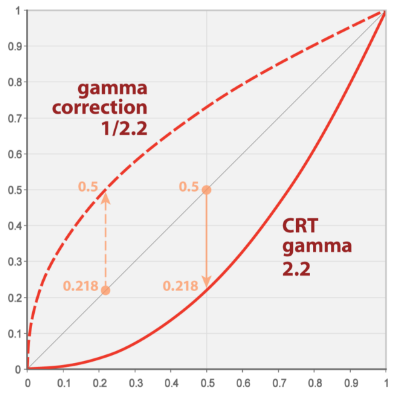
\includegraphics[width=0.35\textwidth]{Lezioni/Immagini/gamma}
	\vspace{-30pt}
\end{wrapfigure}

Il video fornisce informazioni sulla luminosità dell'immagine usando un segnale di luminanza $Y$ ottenuto sommando in modo pesato le componenti RGB, a cui viene in seguito applicata una correzione gamma. 
$$ Y = 0.299R + 0.587G + 0.114B$$
La maggioranza del segnale è composta dal verde; l'informazione colore è codificata in due canali aggiuntivi, ottenuti sottraendo la luminanza dalle componenti rosso e blu.
$$ U = 0.492(B - Y) \qquad V = 0.877(R - Y)$$

Queste due componenti sono chiamate \textbf{chrome}, e la rappresentazione di un valore indipendente dalla luminanza è definita crominanza. 

I coefficienti associati a ogni colore cambiano in base alla posizione geografica per lo standard analogico, mentre per il digitale è globalmente YCrCb. Nella combinazione lineare, il canale più importante è quello del verde. 

I più importanti standard di video analogico sono NTSC in Nord America e Giappone, PAL e SECAM in Europa. I segnali analogici usati sono YUV e YIQ. Le informazioni su colore UV e IQ sono combinate insieme in un segnale di chroma, che a sua volta è combinato con la luminanza Y.

Un altro aspetto da considerare è la \textit{dipendenza tra l'intensità del monitor e la tensione}, la quale ha un fattore esponenziale: il monitor tende a comprimere gli scuri, mostrandoli in livello maggiore.
$$B_d = v_d^{\gamma_d} \qquad \begin{cases}
v_d = \text{tensione} \\
B_d = \text{brightness} \\
\gamma_d = \text{gamma}
\end{cases}$$

Per questo motivo si utilizza la \textbf{gamma correction}, che aumenta l'intensità dei grigi. Essa compensa le caratteristiche di \textbf{non linearità} dei display, per mantenere la compatibilità con i televisori in bianco e nero.

Se il valore del canale rosso è $R$, lo schermo emette una luce proporzionale a $R^\gamma$, con $\gamma \approx 2.2$. In genere il segnale normalizzato viene corretto prima della trasmissione, elevando a $\nicefrac{1}{\gamma}$.

L'HDTV (alta definizione) è concepita per avere una risoluzione doppia rispetto alla TV analogica, con dimensioni in pixel molto più grandi che però permettono l'adattamento agli standard precedenti, aumentando il refresh rate. 

Poiché il sistema visivo è più sensibile all'intensità luminosa che alla croma, si riduce la risoluzione spaziale delle componenti cromatiche. Il campionamento del colore è espresso come $x : y : z$, dove:
\begin{itemize}
	\item $x$ è il numero di campioni di luminanza;
	\item $y$ è il numero dei campioni di chroma per ogni linea dispari;
	\item $z$ è il numero di campioni di chroma per le altre linee.
\end{itemize}

Nella digitalizzazione, i canali Cr e Cb sono di solito campionati orizzontalmente. Lo schema di sottocampionamento $4 : 4 : 4$ indica che non c'è sottocampionamento sulle componenti cromatiche, quindi i valori YCbCr sono tutti trasmessi. 

Per eliminare le coppie, si utilizzano schemi del tipo $4 : 2 : 2$ oppure $4 : 1 : 1$, che trasmettono solamente alcuni valori campionando orizzontalmente. 

 \begin{wrapfigure}{R}{0.4\textwidth}
	\vspace{-20pt}
	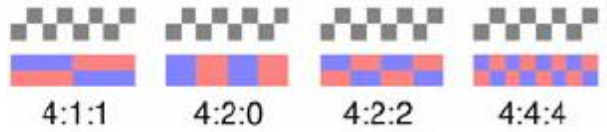
\includegraphics[width=0.4\textwidth]{Lezioni/Immagini/pixel}
	\vspace{-20pt}
\end{wrapfigure}

La compressione JPEG usa $4 : 2 : 0$, il quale elimina un fattore 2 in entrambe le dimensioni posizionando fra righe e colonne un pixel con croma media. Per ogni 4 campioni di luminanza, ci sono 2 chroma sulle linee dispari. 
